\thispagestyle{mainmatter}

\section{Outils d’intégration et de déploiement}
\subsection{GitLab CI}

GitLab CI (Continuous Integration) est un système d’intégration et de livraison continues intégré nativement dans GitLab, une plateforme DevOps complète de gestion du cycle de vie applicatif. Il permet d’automatiser la construction, les tests, la validation, le packaging et le déploiement des applications en s’appuyant sur des pipelines définis de manière déclarative. GitLab CI est aujourd’hui largement utilisé dans les organisations souhaitant industrialiser leurs workflows de développement et renforcer la qualité logicielle.

%point de vue metier
GitLab CI répond à plusieurs enjeux stratégiques  : accélérer le time-to-market, réduire les erreurs humaines, renforcer la traçabilité des changements et améliorer la collaboration entre équipes. Grâce à sa proximité avec le dépôt Git, il apporte une cohérence totale entre le code source, l’historique des commits et les pipelines d’automatisation. Il contribue ainsi à la modernisation et à la professionnalisation des processus de développement.

%point de vue logique et technique
GitLab CI repose sur plusieurs concepts essentiels  :
\begin{itemize}
	\item \textbf{Le fichier .gitlab-ci.yml}  : fichier de configuration déclaratif placé à la racine du dépôt, qui décrit les jobs et les étapes du pipeline.
	\item \textbf{Les jobs}  : unités atomiques qui exécutent des scripts ou des commandes (build, test, deploy).
	\item \textbf{Les stages}  : regroupements logiques des jobs (par exemple, build, test, deploy) exécutés séquentiellement ou en parallèle.
	\item \textbf{Les runners}  : exécutants (machines ou conteneurs) qui traitent les jobs. Ils peuvent être partagés, spécifiques ou autoscalés.
	\item \textbf{Les variables}  : valeurs dynamiques injectées dans les pipelines (clés, secrets, paramètres d’environnement).
	\item \textbf{Les artefacts}  : fichiers générés par les jobs et transmis entre étapes.
\end{itemize}

GitLab CI prend en charge de nombreuses fonctionnalités avancées  : intégration Kubernetes, déclencheurs manuels (manual actions), pipelines multi-projets, stratégies de déploiement progressif et vérification des politiques de sécurité.

\textbf{Exemples et cas d’usage} :
\begin{itemize}
	\item Compiler automatiquement une application dès la création d’une merge request.
	\item Exécuter des tests unitaires et fonctionnels dans un pipeline parallèle.
	\item Formater le code source et analyser les dependences pour détecter les vulnérabilités.
	\item Conteneuriser une application et la pousser vers un registre.
	\item Déployer des applications sur Kubernetes via Helm ou kubectl.
	\item Générer et publier automatiquement la documentation technique.
\end{itemize}

\textbf{Avantages principaux} :
\begin{itemize}
	\item Intégration native avec GitLab et l’ensemble du cycle de vie DevOps.
	\item Modèle déclaratif simple et lisible.
	\item Traçabilité et auditabilité complète des pipelines.
	\item Compatibilité avec les conteneurs et les environnements Kubernetes.
	\item Gestion sécurisée des secrets et des variables sensibles.
	\item Large écosystème de templates, exemples et intégrations communautaires.
\end{itemize}

En synthèse, GitLab CI est une solution stratégique pour automatiser l’intégration et la livraison continues. Il permet aux équipes de gagner en efficacité opérationnelle, d’améliorer la qualité logicielle et d’accélérer la mise en production des innovations.

\textbf{Références et documentations} :
\begin{itemize}
	\item GitLab CI Documentation – \url{https://docs.gitlab.com/ee/ci/}
	\item GitLab CI YAML Reference – \url{https://docs.gitlab.com/ee/ci/yaml/}
	\item GitLab Runners – \url{https://docs.gitlab.com/runner/}
	\item GitLab Kubernetes Integration – \url{https://docs.gitlab.com/ee/user/project/clusters/}
\end{itemize}

\subsection{Commitlint}

Commitlint est un outil open source qui permet de vérifier que les messages de commit respectent un format prédéfini. Il est particulièrement utilisé dans les workflows Git modernes pour renforcer la cohérence des messages de commit, faciliter la génération automatique de changelogs et standardiser la documentation des évolutions logicielles. Commitlint est souvent intégré à des processus de validation automatisés grâce aux hooks Git (par exemple avec Husky) ou aux pipelines CI/CD.

%point de vue metier
Commitlint répond à plusieurs enjeux stratégiques  : améliorer la lisibilité de l’historique des changements, garantir une traçabilité complète des évolutions, renforcer la qualité documentaire et faciliter les audits. La standardisation des messages de commit contribue à instaurer une culture de rigueur et de professionnalisation au sein des équipes de développement.

%point de vue logique et technique
, Commitlint s’appuie sur plusieurs concepts essentiels  :
\begin{itemize}
	\item \textbf{Les règles de validation}  : définissent le format attendu des commits (par exemple, le standard Conventional Commits).
	\item \textbf{Le parser}  : analyse le message de commit et vérifie qu’il correspond au schéma spécifié.
	\item \textbf{La configuration}  : fichier \texttt{commitlint.config.js} où l’on définit les règles, les exceptions et les presets.
	\item \textbf{L’intégration avec Husky}  : permet de déclencher la vérification lors du hook \texttt{commit-msg}.
\end{itemize}

Le standard le plus répandu est \textbf{Conventional Commits}, qui impose un format structuré  :
\begin{verbatim}
<type>(<scope>): <subject>

Exemple :
feat(auth): add JWT authentication
fix(api): handle null pointer exception
docs(readme): update installation instructions
\end{verbatim}

Ce format facilite l’automatisation des versions sémantiques (Semantic Versioning) et la génération des changelogs.

\textbf{Exemples et cas d’usage} :
\begin{itemize}
	\item Empêcher la validation d’un commit si le message ne commence pas par un type valide (ex.: feat, fix, chore).
	\item Bloquer les commits dont le titre dépasse une longueur maximale.
	\item Valider automatiquement tous les messages de commit dans un pipeline CI/CD.
	\item Générer des changelogs structurés à partir des commits normalisés.
	\item Appliquer un format de commit homogène sur plusieurs équipes et projets.
\end{itemize}

\textbf{Avantages principaux} :
\begin{itemize}
	\item Standardisation et lisibilité accrue des messages de commit.
	\item Réduction des erreurs et des incohérences documentaires.
	\item Automatisation des processus de release et de génération de changelogs.
	\item Compatibilité avec les pratiques GitOps et CI/CD.
	\item Facilité d’intégration avec Husky et d’autres outils de hooks Git.
\end{itemize}

En synthèse, Commitlint est une brique essentielle pour industrialiser et professionnaliser la gestion des versions et la documentation des projets logiciels. Il contribue à instaurer une culture DevOps rigoureuse et à améliorer la traçabilité du cycle de développement.

\textbf{Références suggérées} :
\begin{itemize}
	\item Commitlint Documentation – \url{https://commitlint.js.org/}
	\item Conventional Commits – \url{https://www.conventionalcommits.org/}
	\item Husky Documentation – \url{https://typicode.github.io/husky/}
	\item Semantic Versioning – \url{https://semver.org/}
	\item GitHub Commitlint Repository – \url{https://github.com/conventional-changelog/commitlint}
\end{itemize}

\subsection{Husky}

Husky est un outil open source permettant de gérer et d’exécuter des hooks Git de manière simple et centralisée dans les projets logiciels. Il facilite l’automatisation de tâches de validation et de mise en conformité lors des événements Git, tels que les commits, les pushs ou les merges. Grâce à sa configuration déclarative, Husky contribue à instaurer des pratiques DevOps rigoureuses et à renforcer la qualité du code tout au long du cycle de développement.

%point de vue metier
Husky répond à plusieurs enjeux stratégiques  : réduire les erreurs humaines, homogénéiser les workflows entre équipes, accélérer le feedback lors des validations et améliorer la traçabilité des changements. Il constitue un levier essentiel de professionnalisation, car il garantit que les standards de qualité (tests, linting, conventions de commit) sont systématiquement respectés avant d’intégrer le code au référentiel principal.

%point de vue logique et technique
, Husky repose sur plusieurs concepts clés  :
\begin{itemize}
	\item \textbf{Les hooks Git}  : scripts déclenchés automatiquement par Git à différents moments du cycle de vie (par exemple \texttt{pre-commit}, \texttt{commit-msg}, \texttt{pre-push}).
	\item \textbf{La configuration}  : Husky utilise des commandes déclarées dans le fichier \texttt{package.json} ou dans des fichiers dédiés (\texttt{.husky/pre-commit}).
	\item \textbf{Les intégrations}  : Husky fonctionne avec de nombreux outils tels que ESLint, Prettier, Commitlint ou les tests unitaires.
	\item \textbf{Le workflow Node.js}  : bien qu’installé via npm ou Yarn, Husky est indépendant du langage utilisé dans le projet.
\end{itemize}

Les hooks les plus fréquemment utilisés sont  :
\begin{itemize}
	\item \texttt{pre-commit}  : exécute des validations avant l’enregistrement d’un commit (linting, tests).
	\item \texttt{commit-msg}  : vérifie que le message de commit respecte une convention donnée.
	\item \texttt{pre-push}  : lance des vérifications avant l’envoi du code sur le dépôt distant.
\end{itemize}

\textbf{Exemples et cas d’usage} :
\begin{itemize}
	\item Lancer ESLint automatiquement sur les fichiers modifiés avant chaque commit.
	\item Exécuter Commitlint pour garantir que les messages de commit respectent Conventional Commits.
	\item Vérifier que les tests unitaires passent avant chaque push.
	\item Appliquer Prettier pour uniformiser le formatage du code source.
	\item Refuser les commits contenant des erreurs de syntaxe ou de style.
	\item Exécuter des scripts personnalisés pour valider des règles métier spécifiques.
	\item Executer des scripts de sécurité pour détecter les vulnérabilités dans les dépendances.
	\item Vérifier que les fichiers de configuration sont à jour , conformes aux standards et ne contiennent pas d'informations sensibles.
	\item Bloquer la création de commits vides ou sans description.
\end{itemize}

\textbf{Avantages principaux} :
\begin{itemize}
	\item Standardisation des processus de validation dans toute l’équipe.
	\item Réduction des erreurs humaines et des régressions en amont des CI/CD.
	\item Facilité de mise en œuvre et de configuration.
	\item Compatibilité avec de nombreux outils de qualité logicielle.
	\item Exécution rapide et locale, sans dépendre de l’environnement distant.
\end{itemize}

En synthèse, Husky est un composant essentiel pour fiabiliser et automatiser les workflows de validation des projets modernes. Il contribue à instaurer une culture DevOps orientée qualité et à renforcer la cohérence entre les contributeurs.

\textbf{Références suggérées} :
\begin{itemize}
	\item Husky Documentation – \url{https://typicode.github.io/husky/}
	\item Git Hooks Documentation – \url{https://git-scm.com/docs/githooks}
	\item Commitlint Documentation – \url{https://commitlint.js.org/}
	\item ESLint Documentation – \url{https://eslint.org/docs/latest/}
	\item Prettier Documentation – \url{https://prettier.io/docs/en/}
\end{itemize}

\textbf{Références suggérées supplémentaires pour la sécurité du code} :
\begin{itemize}
	\item npm Audit Documentation – \url{https://docs.npmjs.com/cli/v10/commands/npm-audit}
	\item Snyk Documentation – \url{https://docs.snyk.io/}
	\item Trivy Documentation – \url{https://aquasecurity.github.io/trivy/}
	\item OWASP Dependency-Check – \url{https://jeremylong.github.io/DependencyCheck/}
	\item Bandit Documentation – \url{https://bandit.readthedocs.io/en/latest/}
\end{itemize}

\subsection{Semantic Release}

Semantic Release est un outil open source qui automatise le versionnement et la publication des packages logiciels en s’appuyant sur les messages de commit et le principe du versionnement sémantique (Semantic Versioning). Il supprime le besoin de mise à jour manuelle du numéro de version et de rédaction des changelogs, contribuant ainsi à la fiabilisation et à l’industrialisation des processus de release.

%point de vue metier
Semantic Release répond à plusieurs enjeux stratégiques  : réduire les erreurs humaines dans les versions publiées, accélérer le cycle de livraison, renforcer la traçabilité des évolutions et homogénéiser les workflows de publication entre équipes. En automatisant intégralement la release, il permet aux développeurs de se concentrer sur la qualité fonctionnelle plutôt que sur les tâches administratives.

%point de vue logique et technique
, Semantic Release repose sur plusieurs concepts clés  :
\begin{itemize}
	\item \textbf{Les conventions de commit}  : le projet s’appuie sur des formats structurés (par exemple Conventional Commits) pour déduire automatiquement l’impact des changements (correctifs, nouvelles fonctionnalités, breaking changes).
	\item \textbf{Le calcul automatique de la version}  : en fonction des types de commits depuis la dernière release, Semantic Release incrémente la version majeure, mineure ou corrective.
	\item \textbf{La génération du changelog}  : compilation automatique des changements pertinents dans un format lisible.
	\item \textbf{La publication}  : déploiement automatisé vers les registres de packages (npm, Maven, Docker Hub) et création des tags Git correspondants.
\end{itemize}

Semantic Release s’intègre naturellement dans des pipelines CI/CD (GitHub Actions, GitLab CI, CircleCI), garantissant que chaque merge dans la branche principale déclenche la création d’une nouvelle version stable.

\textbf{Exemples et cas d’usage} :
\begin{itemize}
	\item Publier automatiquement un package npm lorsque de nouvelles fonctionnalités sont mergées.
	\item Générer un changelog détaillé à partir des commits, sans intervention manuelle.
	\item Tagger les versions dans Git et créer des releases GitHub avec les notes correspondantes.
	\item Déclencher un pipeline de build Docker et pousser l’image versionnée sur un registre.
	\item Refuser les releases en cas de non-respect des conventions de commit.
\end{itemize}

\textbf{Avantages principaux} :
\begin{itemize}
	\item Automatisation complète et fiabilisée du cycle de versionnement et de publication.
	\item Réduction drastique des erreurs humaines et des oublis dans la gestion des versions.
	\item Traçabilité et transparence accrues grâce aux changelogs générés automatiquement.
	\item Compatibilité avec de nombreux systèmes CI/CD et écosystèmes de packaging.
	\item Homogénéité des pratiques de release entre les projets et les équipes.
\end{itemize}

En synthèse, Semantic Release est une solution stratégique pour les organisations souhaitant industrialiser et sécuriser leur processus de publication. Il apporte une cohérence et une rapidité qui renforcent la qualité et la crédibilité des livraisons logicielles.

\textbf{Références suggérées} :
\begin{itemize}
	\item Semantic Release Documentation – \url{https://semantic-release.gitbook.io/}
	\item Conventional Commits – \url{https://www.conventionalcommits.org/}
	\item Semantic Versioning – \url{https://semver.org/}
	\item GitHub Actions Documentation – \url{https://docs.github.com/en/actions}
	\item npm Publishing Guide – \url{https://docs.npmjs.com/creating-and-publishing-unscoped-public-packages}
\end{itemize}
\section{Les conventions de commits}

Les conventions de commits désignent l’ensemble des règles et des bonnes pratiques qui encadrent la rédaction des messages de commit dans un système de gestion de versions (comme Git). Elles visent à standardiser la documentation des changements, à faciliter la compréhension de l’historique d’un projet et à automatiser certaines tâches (génération de changelogs, déclenchement de pipelines CI/CD, versionnement sémantique). Leur adoption contribue à renforcer la qualité des projets logiciels et la collaboration entre les équipes.

%point de vue metier
les conventions de commits permettent de valoriser la traçabilité et la lisibilité du code. Elles facilitent la revue des changements lors des audits, améliorent la communication entre développeurs et garantissent que l’évolution du produit est documentée de façon claire et structurée. Elles sont également un levier de professionnalisation et de crédibilité vis-à-vis des partenaires et des clients, qui attendent des processus de développement rigoureux et transparents.

%point de vue logique et technique
, plusieurs standards de conventions ont émergé, notamment :
\begin{itemize}
	\item \textbf{Conventional Commits} : une spécification populaire qui définit un format structuré basé sur des préfixes et des catégories. Exemple :
	      \begin{verbatim}
    feat(auth): add JWT authentication
    fix(api): correct error handling in user service
    docs(readme): update installation instructions
	      \end{verbatim}
	\item \textbf{Semantic Versioning} : combiné aux conventions de commits, il permet de déclencher automatiquement les incréments de version (MAJOR, MINOR, PATCH) selon la nature des changements.
	\item \textbf{Gitmoji} : l’usage d’emojis standardisés pour symboliser visuellement le type de modification :
	      \begin{verbatim}
    eat: add search functionality
    fix: resolve crash on startup
    docs: improve API documentation
	      \end{verbatim}
\end{itemize}

Les conventions de commits permettent d’automatiser des processus critiques :
\begin{itemize}
	\item Génération de changelogs clairs à partir des messages structurés.
	\item Déclenchement de pipelines CI/CD conditionnés à certains types de changements.
	\item Application automatique de politiques de versionnement.
	\item Vérification des formats de message via des hooks Git (ex. Commitlint).
\end{itemize}

\textbf{Exemples et cas d’usage} :
\begin{itemize}
	\item Utiliser la convention Conventional Commits pour tous les projets d’un département afin de générer automatiquement la documentation des versions.
	\item Configurer un pipeline CI/CD qui refuse les commits non conformes au format attendu.
	\item Associer des préfixes (feat, fix, chore) aux incréments automatiques de version selon Semantic Versioning.
	\item Appliquer des tags de breaking change via l’indication \texttt{BREAKING CHANGE} dans le corps du commit.
\end{itemize}

\textbf{Avantages principaux} :
\begin{itemize}
	\item Lisibilité et compréhension accrues de l’historique des changements.
	\item Automatisation de la génération des notes de version et du versionnement.
	\item Réduction des erreurs humaines grâce aux validations automatiques.
	\item Amélioration de la collaboration et de la revue de code.
	\item Renforcement de la transparence et de la traçabilité du cycle de développement.
\end{itemize}

En synthèse, l’adoption de conventions de commits structurées ne constitue pas uniquement une formalité : elle participe pleinement à l’industrialisation et à la qualité des processus de développement logiciel. Elle s’inscrit dans une démarche globale d’automatisation, de traçabilité et de professionnalisation des projets.

\textbf{Références suggérées} :
\begin{itemize}
	\item Conventional Commits Specification – \url{https://www.conventionalcommits.org/}
	\item Semantic Versioning – \url{https://semver.org/}
	\item Gitmoji – \url{https://gitmoji.dev/}
	\item Pro Git Book – \url{https://git-scm.com/book/en/v2}
	\item Gousios, G., Spinellis, D. (2012). GIT-EVOLVE: A Software Evolution Tool Based on Git.
\end{itemize}

\section{Mise en place des pipelines CI/CD}

La mise en place d’une chaîne CI/CD (Continuous Integration / Continuous Deployment) constitue un levier essentiel pour automatiser la construction, le test et le déploiement des applications.
Ce processus contribue à réduire les délais de mise en production, à limiter les erreurs humaines et à fiabiliser les évolutions logicielles.

\subsection{Conteneurisation des applications}

La première étape du pipeline CI/CD consiste à conteneuriser les applications développées.
Pour ce faire, des fichiers \texttt{Dockerfile} ont été créés pour chaque projet, décrivant :
\begin{itemize}
	\item Le système de base à utiliser (par exemple \texttt{python:3.10-slim}, \texttt{node:lts}).
	\item L’installation des dépendances applicatives via \texttt{pip}, \texttt{npm} ou autres gestionnaires de paquets.
	\item La copie du code source et des fichiers de configuration.
	\item La définition du point d’entrée de l’application (\texttt{ENTRYPOINT}).
\end{itemize}

Cette approche garantit que chaque build produit une image identique, facilement transportable et exécutable dans tout environnement Kubernetes.

\subsection{Tagging des images}

Le tagging des images conteneurisées ne peut pas être aléatoire, car il constitue la base de la traçabilité, de la reproductibilité et de la fiabilité des déploiements. Un schéma de versionnement clair et systématique permet de relier chaque image à son origine exacte et d'éviter toute ambiguïté lors des mises en production.

Tout d'abord, l'utilisation d'un tag unique garantit la \textbf{traçabilité stricte}. Par exemple, lorsqu'un incident survient en production, il est indispensable de savoir précisément quel code source a généré l'image déployée. Si les tags étaient choisis de manière arbitraire ou remplacés sans cohérence (par exemple avec \texttt{latest} écrasé à chaque build), il serait impossible de retrouver la version exacte à l'origine du problème.

Ensuite, un tagging rigoureux assure la \textbf{reproductibilité des environnements}. Lorsqu'un même tag est utilisé dans différents clusters (staging, production), il doit toujours pointer vers la même image. Ainsi, un déploiement appliqué plusieurs semaines plus tard avec le même manifeste Kubernetes sera identique au déploiement initial. Sans cette convention, des différences imprévisibles pourraient introduire des comportements inattendus.

Le schéma de versionnement facilite également le \textbf{rollback} en cas de défaillance. Si une nouvelle version introduit un bug critique, il est possible de restaurer immédiatement l'image antérieure en redeployant le tag correspondant (par exemple \texttt{v1.2.3-main}), sans incertitude sur son contenu.

Enfin, cette approche contribue à la \textbf{sûreté des opérations et à l'auditabilité}. Dans des contextes soumis à des exigences réglementaires (ISO, PCI-DSS) ou à des politiques internes strictes, le tag constitue une preuve technique qui relie chaque binaire à son processus de fabrication (pipeline CI/CD) et à son commit d'origine. Il devient ainsi possible de démontrer qui a produit l'image, à quel moment et avec quelles sources.

Ces cas d'usage illustrent qu'un schéma de tagging structuré est essentiel pour garantir la qualité, la sécurité et la maîtrise des déploiements en environnement conteneurisé.

Le versionnement des images conteneurisées est essentiel pour assurer la traçabilité des déploiements.
Les pipelines CI/CD ont été configurés pour appliquer un schéma de tagging cohérent :
\begin{itemize}
	\item Utilisation d’un tag unique basé sur le hash du commit Git.
	\item Création d’un tag lisible incluant le numéro de version et la branche (par exemple \texttt{v1.2.3-main}).
	\item Marquage automatique de l’image la plus récente comme \texttt{latest} pour simplifier les tests.
\end{itemize}

Ces conventions permettent de relier chaque déploiement Kubernetes à l’image exacte qui a été produite par la pipeline.

\subsection{Configuration de l’authentification}

La sécurité des échanges entre les outils CI/CD et les services externes (registre d’images, dépôt GitOps) repose sur une gestion rigoureuse des identifiants et des autorisations.

Plusieurs mesures ont été mises en œuvre pour garantir une authentification sécurisée :
\begin{itemize}
	\item Création de comptes de service dédiés avec des droits limités.
	\item Génération de tokens d’accès spécifiques à chaque usage.
	\item Stockage sécurisé des identifiants et des tokens via les \textbf{variables GitLab CI/CD}, marquées comme protégées et masquées.
	\item Définition de règles de rotation périodique de ces secrets.
\end{itemize}

\subsection{Authentification CI/CD vers Harbor (registre d’images)}

Les runners GitLab doivent pouvoir pousser les images Docker construites vers Harbor.

\subsection{Étapes de configuration}

La création d’un compte robot dans Harbor constitue une étape essentielle afin de permettre l’automatisation des interactions avec le registre d’images. Ce mécanisme s’avère particulièrement utile dans le cadre d’une chaîne DevOps, notamment pour les processus de déploiement continu et la gestion des artefacts.

Dans le cadre de ce projet, la configuration a débuté par l’accès au projet ciblé au sein de l’interface web de Harbor. Ce projet regroupe les dépôts d’images Docker concernés par l’automatisation. La figure suivante illustre l’écran correspondant :

\begin{figure}[H]
	\centering
	\includegraphics[width=0.6\textwidth]{figures/projet ciblé.png}
	\caption{Accès au projet ciblé sur Harbor}
\end{figure}

La création du compte robot a ensuite été initiée via l’onglet Robot Accounts, par la sélection de l’option New Robot Account. Cette action ouvre un formulaire structuré en plusieurs sections. Dans la première section, des informations générales sont renseignées, telles que le nom du compte et une description précisant son rôle. La possibilité de définir une date d’expiration est également proposée, de manière à limiter la durée de validité de l’accès, conformément aux bonnes pratiques de sécurité.

\begin{figure}[H]
	\centering
	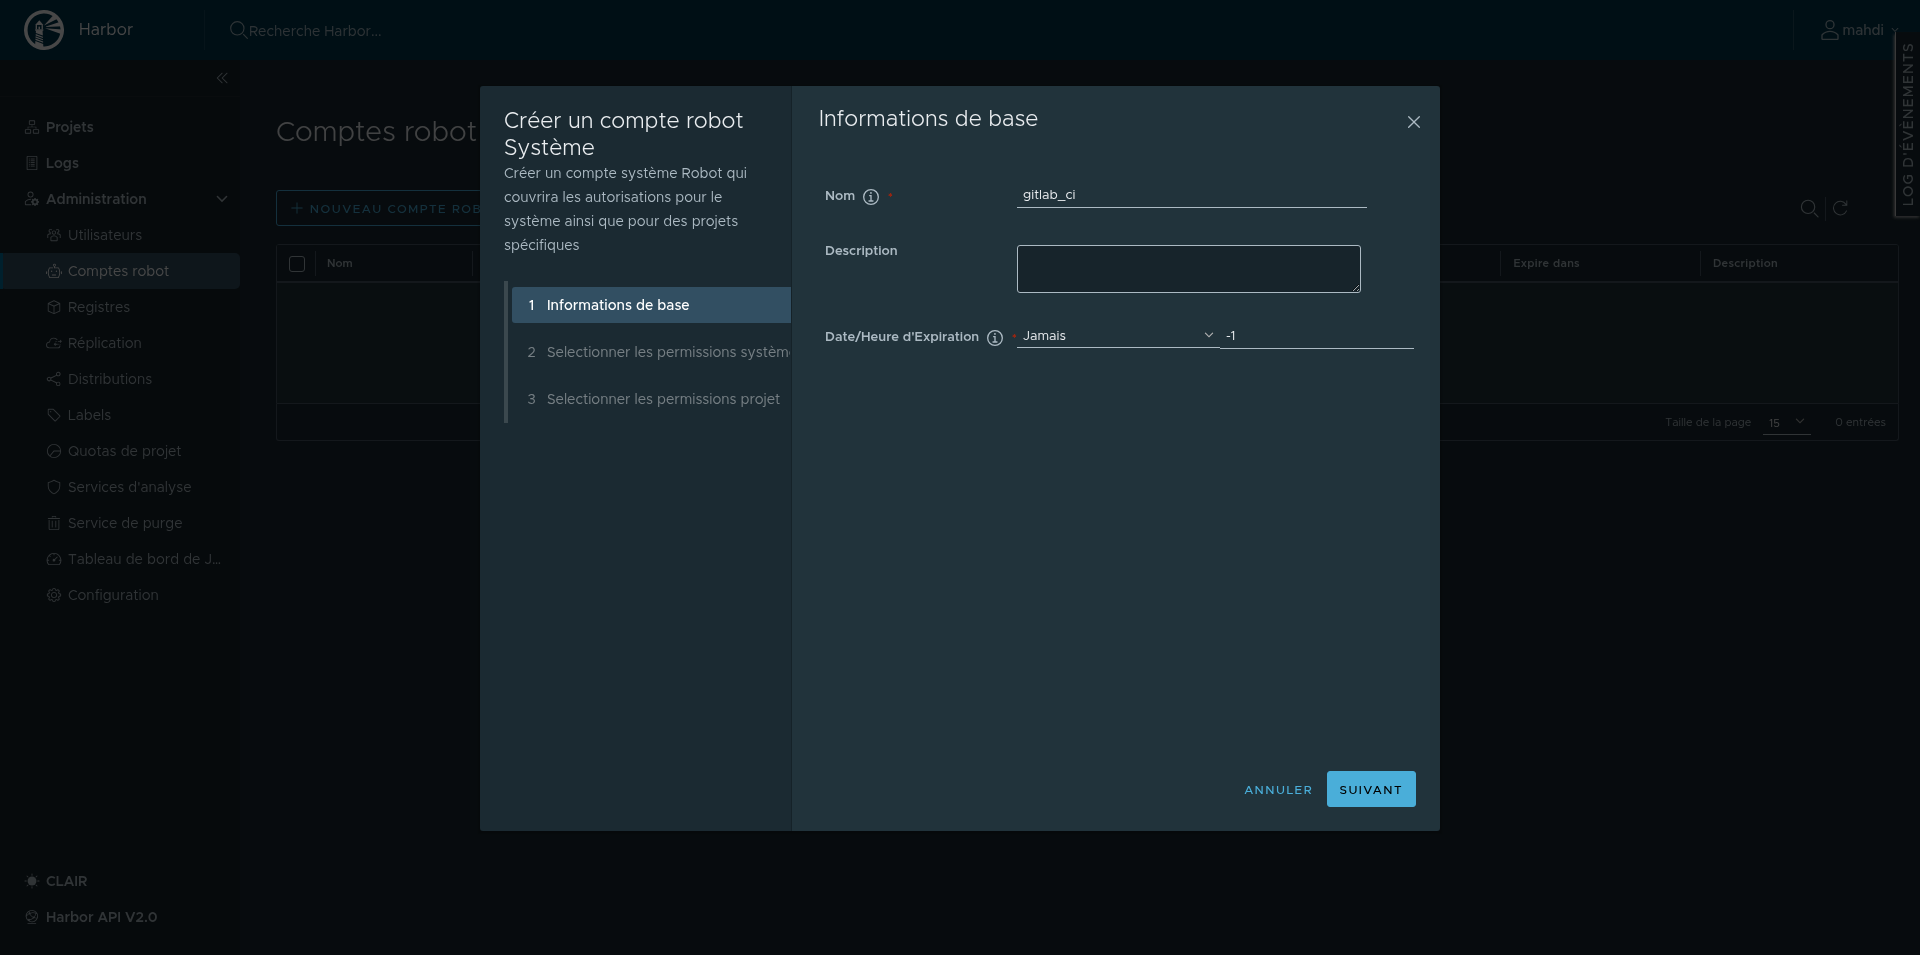
\includegraphics[width=0.6\textwidth]{figures/harbor robot account informations de base.png}
	\caption{Paramètres de base du compte robot}
\end{figure}

La configuration des permissions système, illustrée ci-dessous, permet de spécifier des droits d’administration globaux. Dans le présent contexte, ces permissions n’ont pas été activées, le compte devant uniquement intervenir au niveau d’un projet spécifique.

\begin{figure}[H]
	\centering
	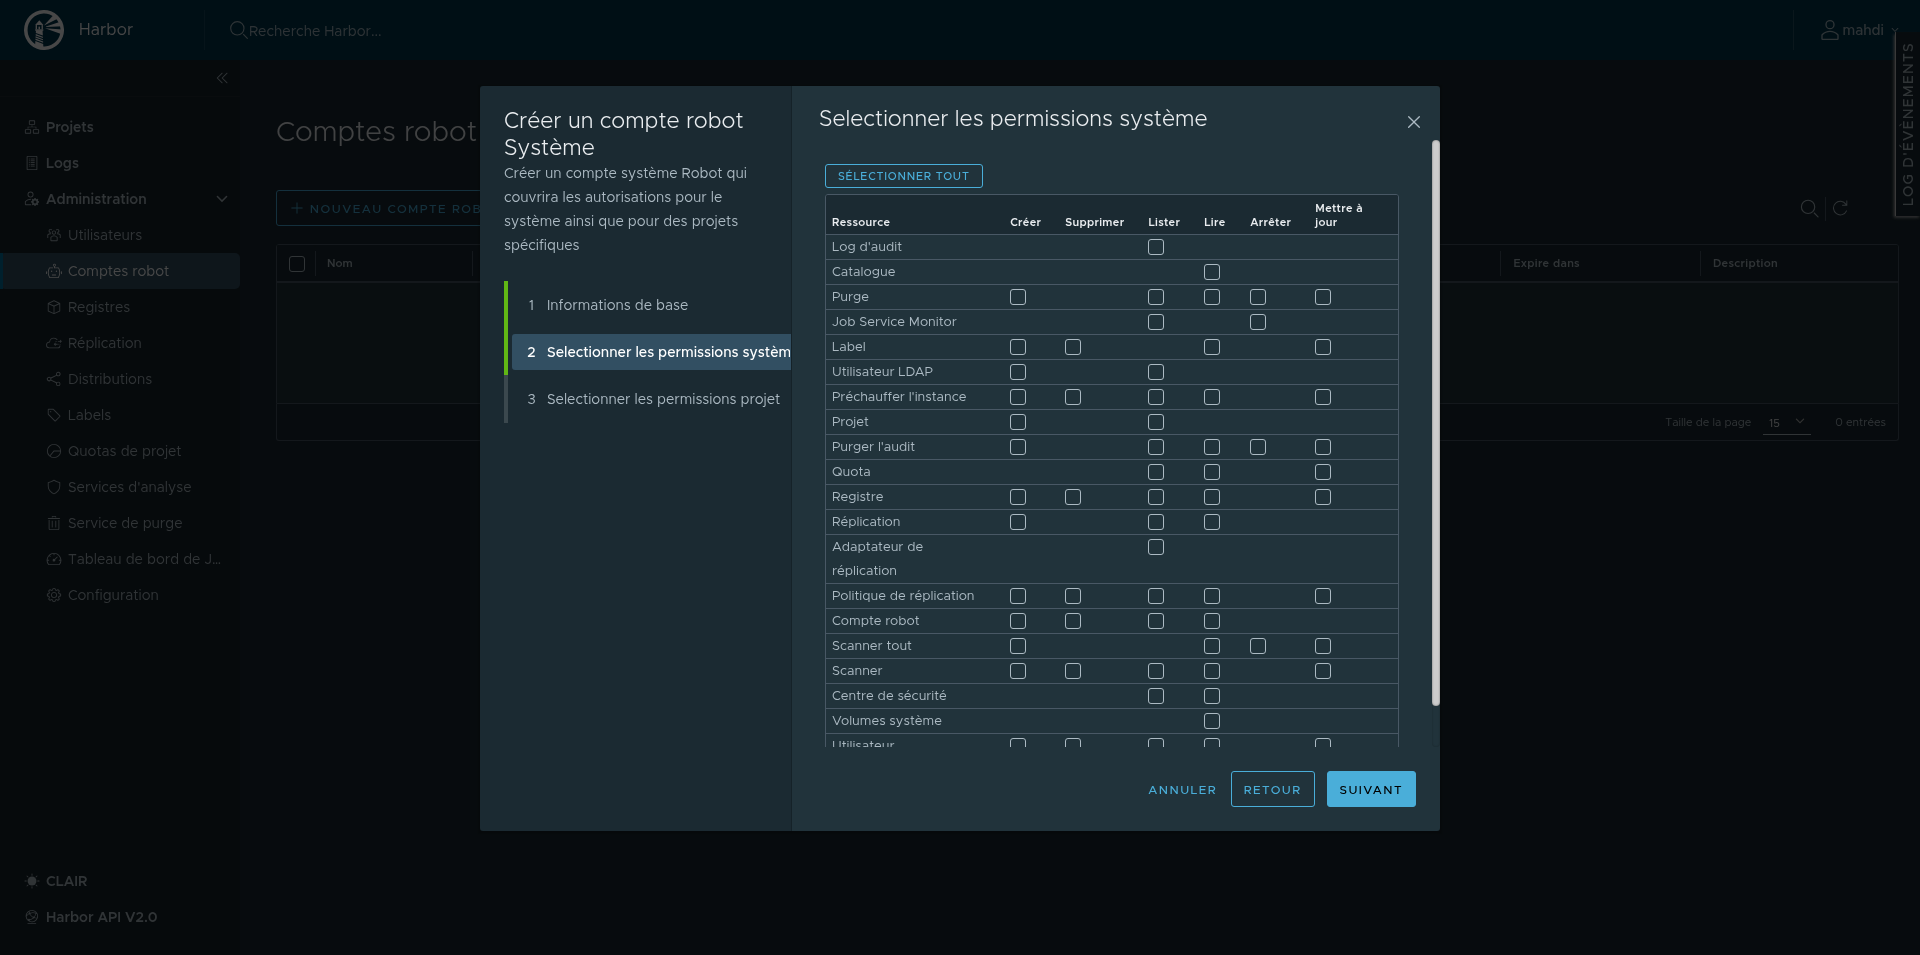
\includegraphics[width=0.6\textwidth]{figures/harbor robot account permissions systeme.png}
	\caption{Configuration des permissions système}
\end{figure}

La sélection des projets associés s’effectue ensuite, en précisant les espaces sur lesquels le compte robot pourra opérer.

\begin{figure}[H]
	\centering
	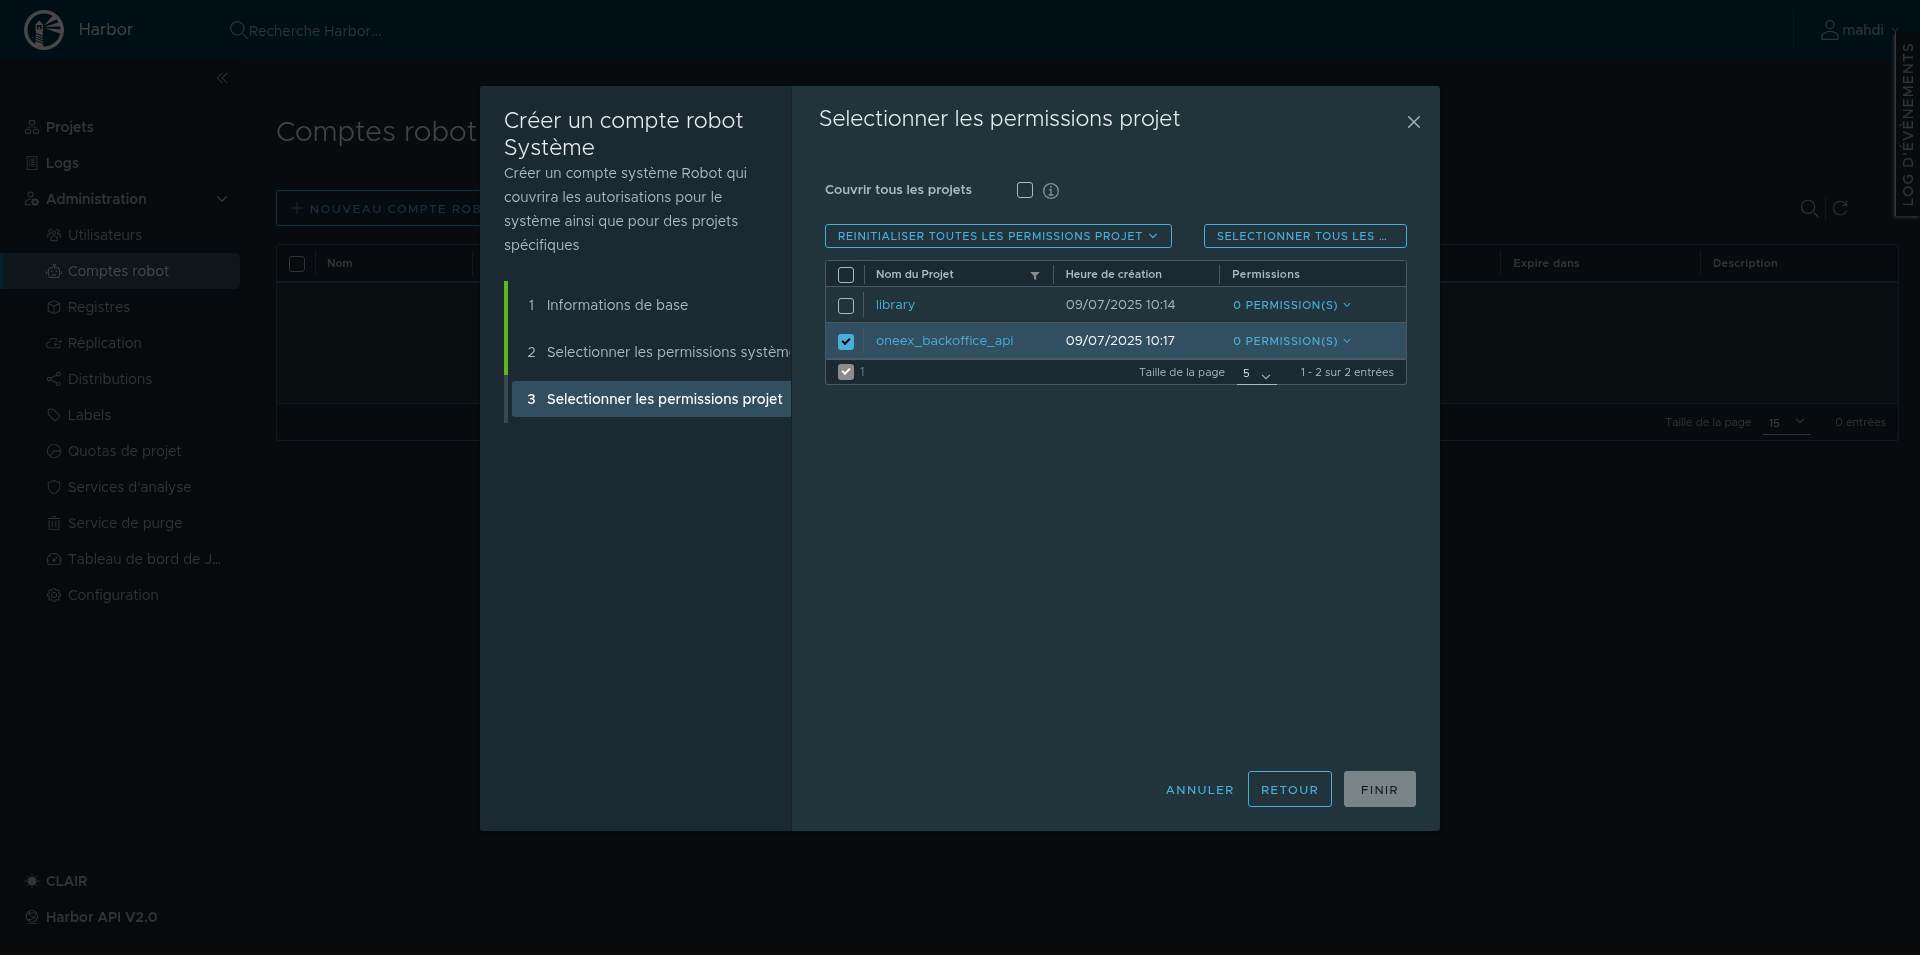
\includegraphics[width=0.6\textwidth]{figures/harbor robot account projects.png}
	\caption{Sélection des projets cibles}
\end{figure}

Pour chaque projet, des permissions détaillées sont définies. Dans cette configuration, le compte a été autorisé à créer et lister des images, à visualiser les journaux et les rapports de vulnérabilités (CVE), ainsi qu’à créer, supprimer et lister des tags. Cette granularité des droits vise à garantir que toutes les images soient correctement identifiées, tout en permettant la suppression des tags obsolètes et la supervision des éventuels problèmes de sécurité.

\begin{figure}[H]
	\centering
	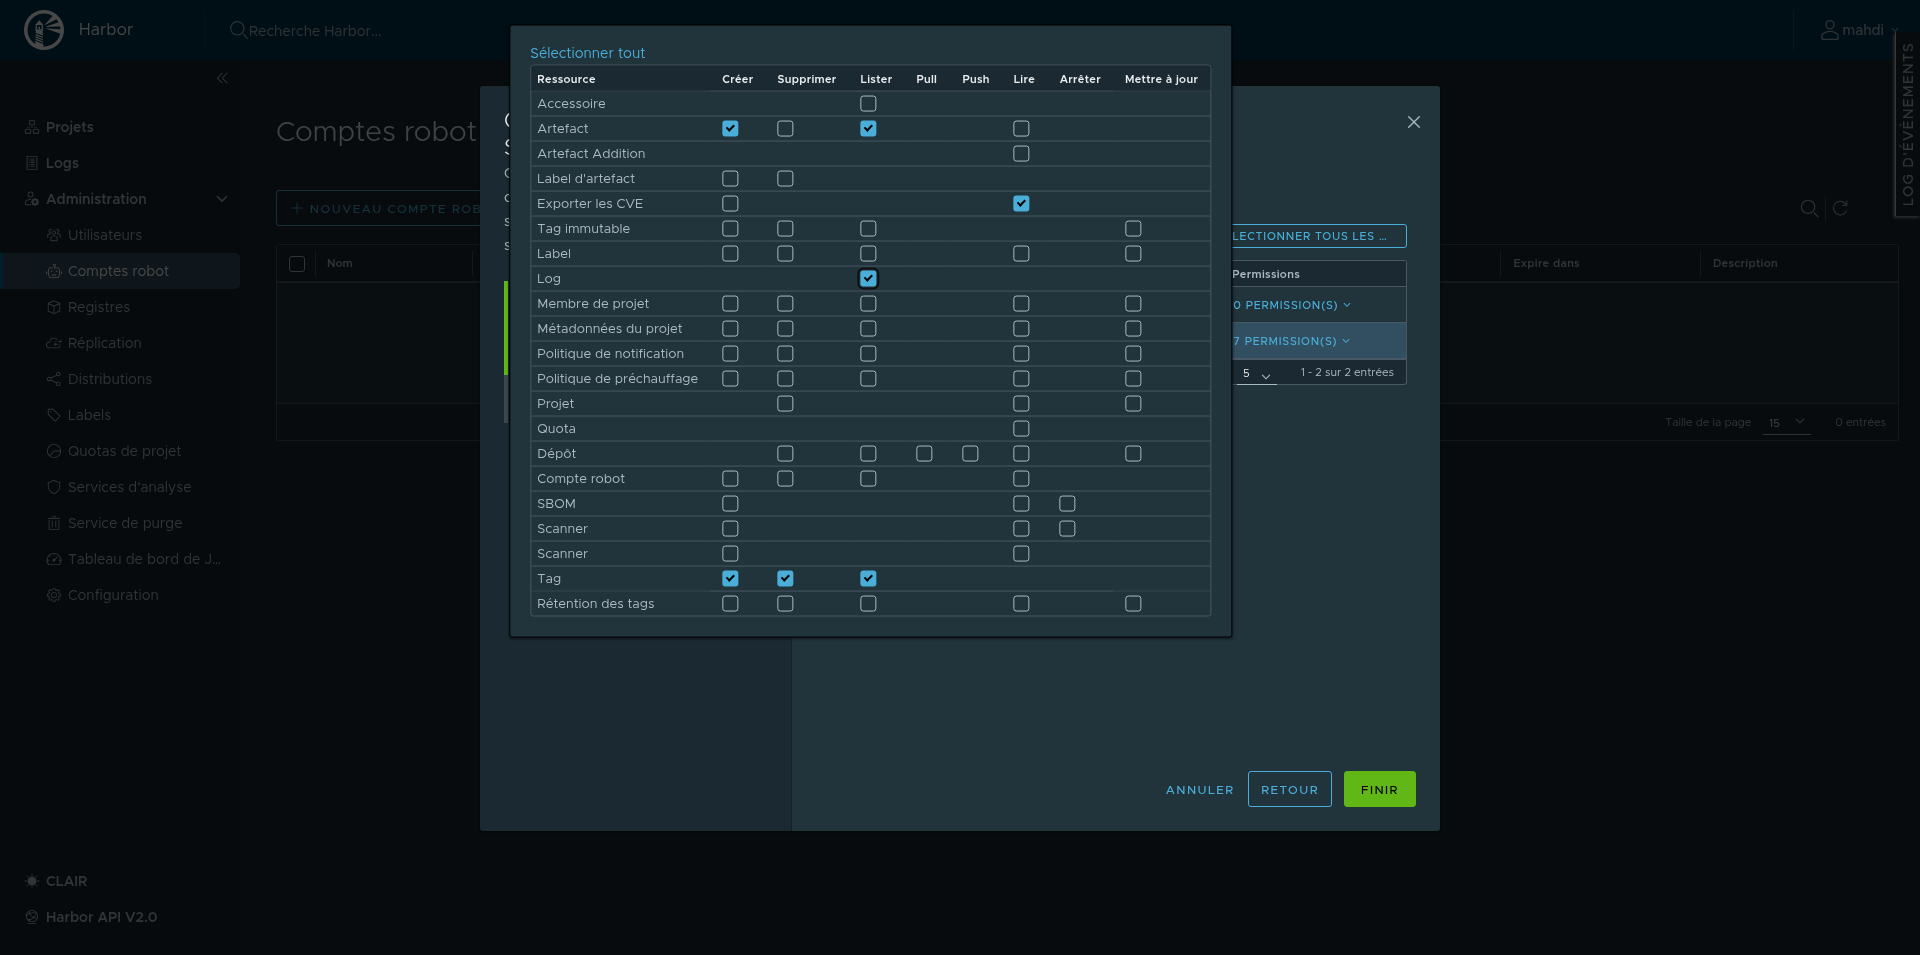
\includegraphics[width=0.6\textwidth]{figures/harbor robot account projects permissions.png}
	\caption{Définition des permissions spécifiques aux projets}
\end{figure}

Une fois les paramètres configurés, l’activation du compte et la génération du jeton d’authentification sont effectuées en cochant respectivement les options Activer le compte Robot et Générer un nouveau jeton. Le jeton généré est présenté à l’issue de l’opération. Il est important de noter que ce jeton constitue un identifiant unique et confidentiel, utilisé pour authentifier les requêtes automatisées. Il doit être conservé de manière sécurisée, puisqu’il ne peut pas être récupéré ultérieurement via l’interface.

\begin{figure}[H]
	\centering
	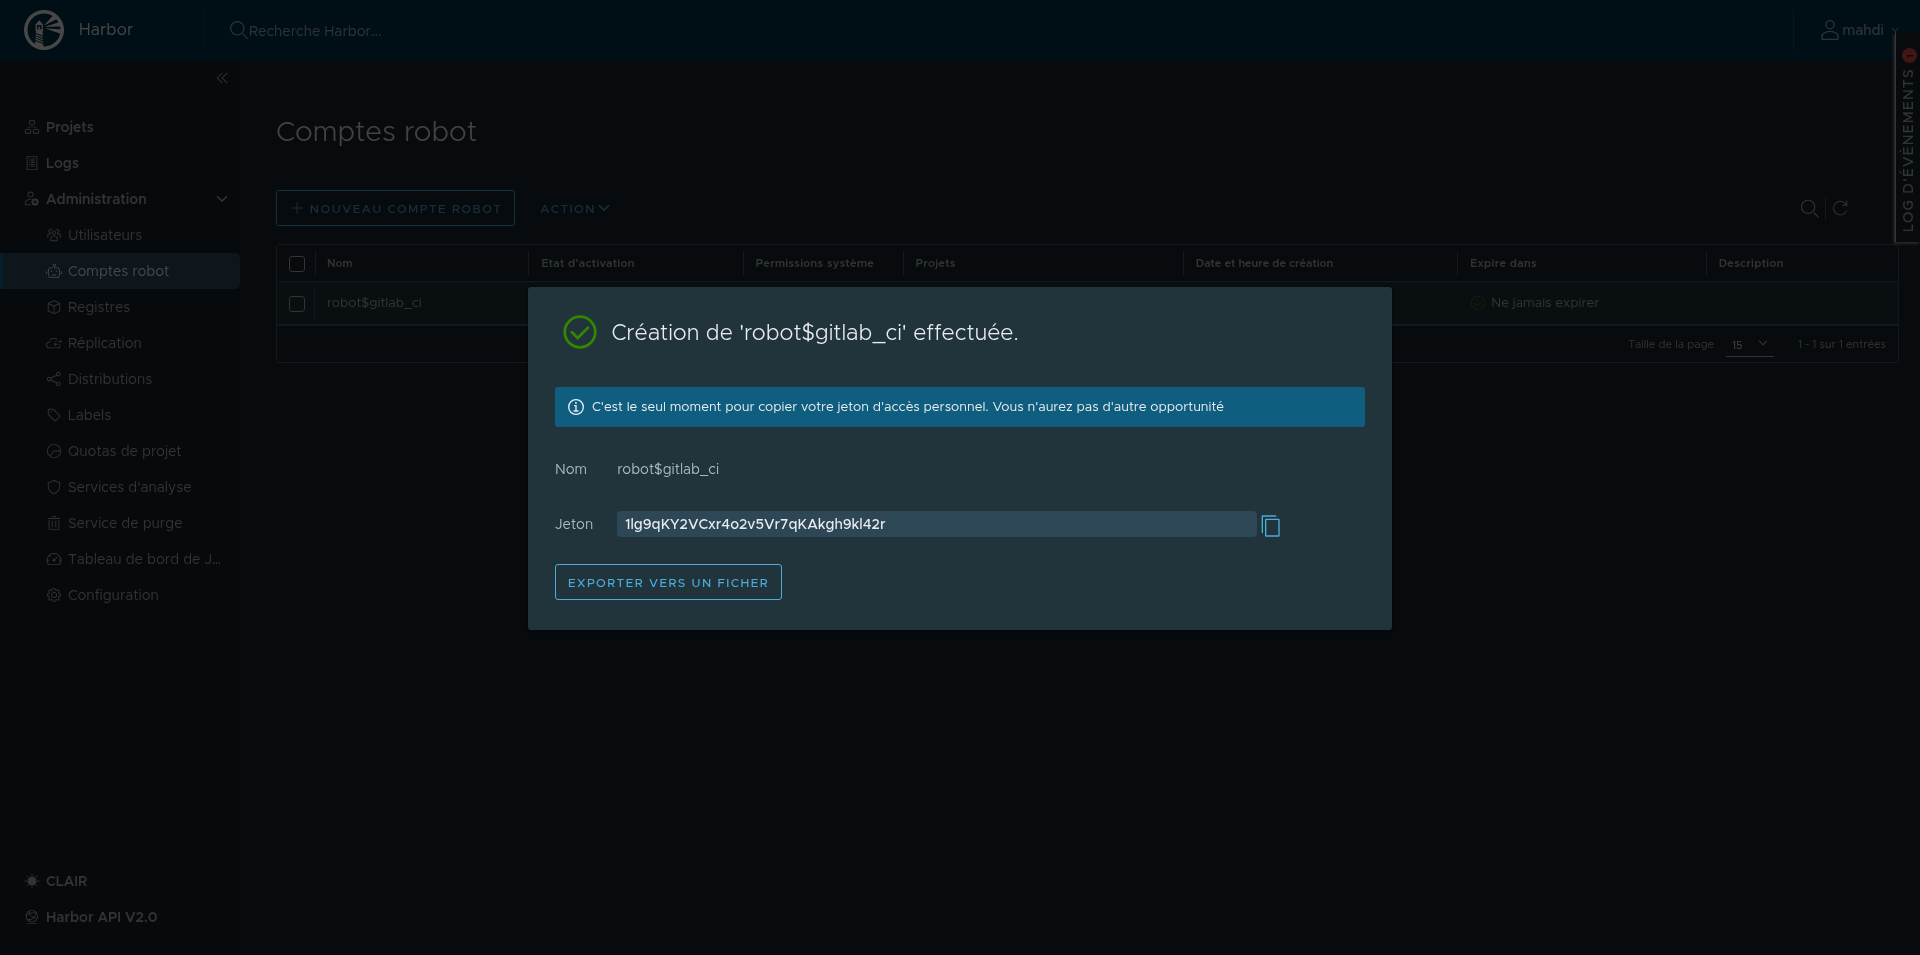
\includegraphics[width=0.6\textwidth]{figures/harbor robot account jeton.png}
	\caption{Jeton généré pour le compte robot}
\end{figure}

L’ensemble de ces étapes permet de disposer d’un compte robot configuré de façon fine et conforme aux besoins du projet, garantissant à la fois la sécurité et la traçabilité des opérations automatisées sur le registre Harbor.

La seconde étape consiste à configurer le \emph{GitLab Runner} afin qu’il puisse interagir de manière sécurisée avec le registre Harbor, notamment pour réaliser l’authentification et le dépôt automatique des images Docker construites au cours des pipelines CI/CD.

Dans un premier temps, les identifiants nécessaires à l’authentification ont été ajoutés sous forme de variables de projet GitLab. Cette opération s’effectue via l’interface web de GitLab, dans le menu \emph{Settings > CI/CD > Variables}, tel qu’illustré ci-dessous :

\begin{figure}[H]
	\centering
	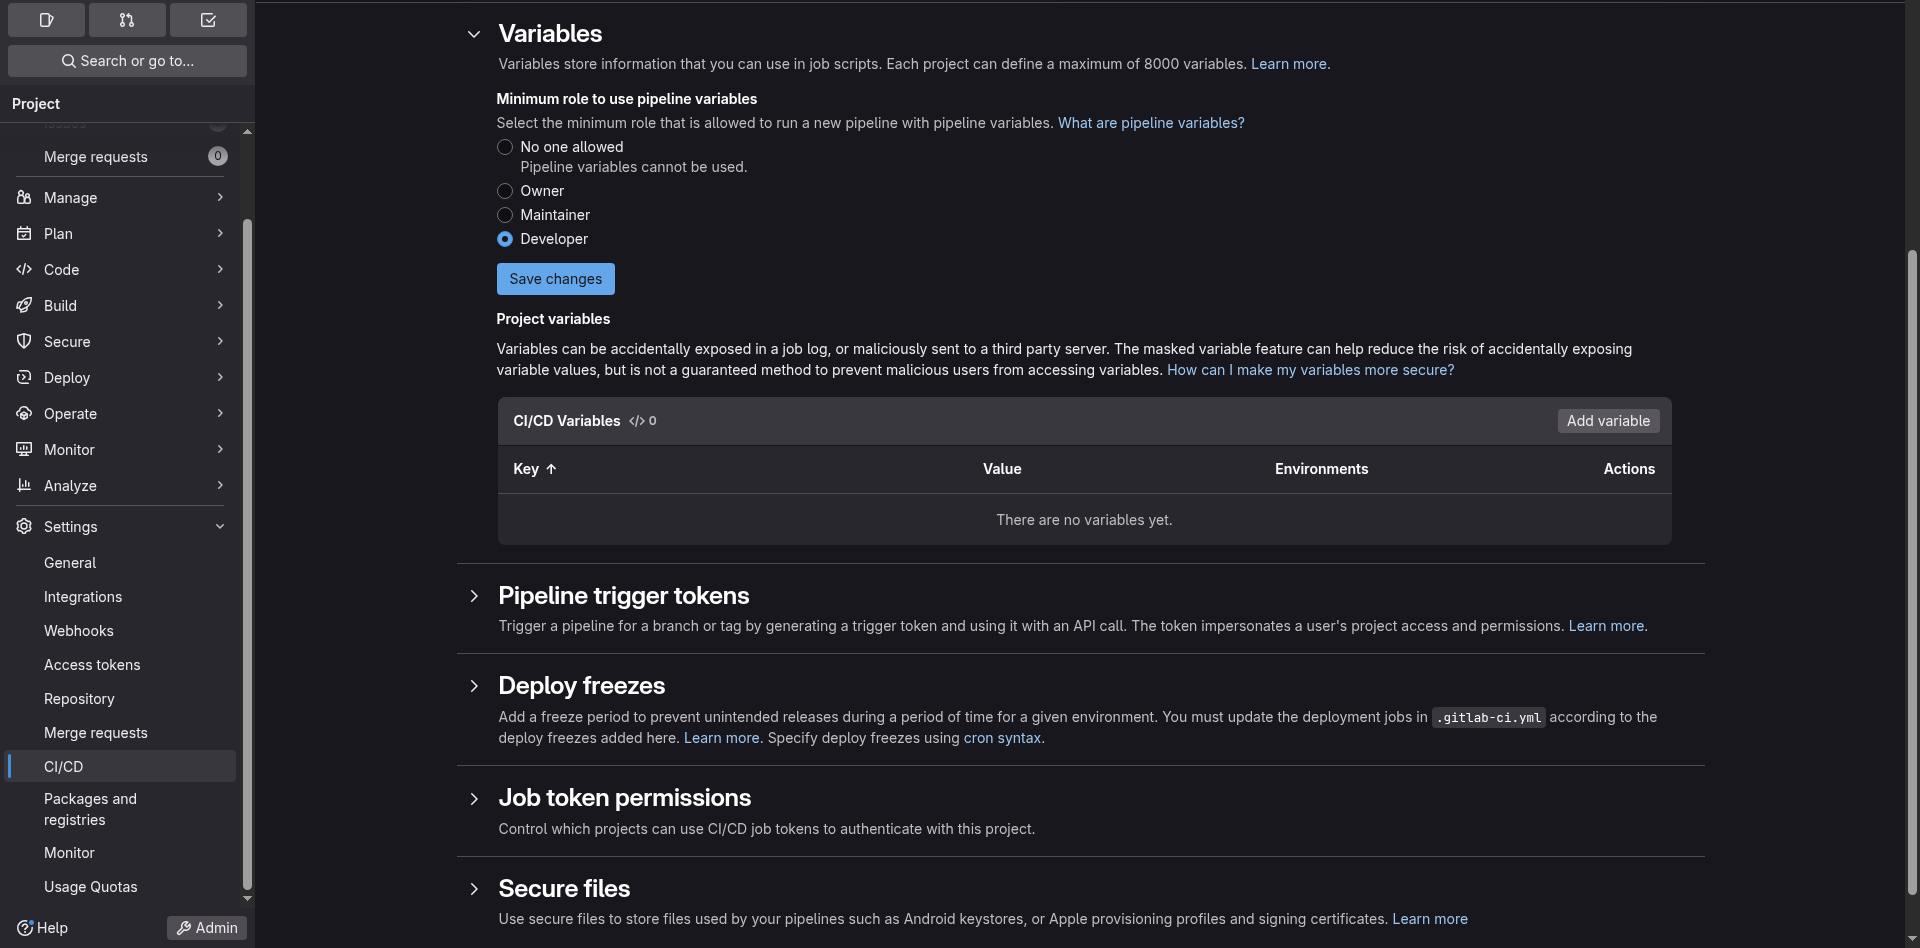
\includegraphics[width=0.65\textwidth]{figures/gitlab variables menu.png}
	\caption{Accès aux variables CI/CD dans l’interface GitLab}
\end{figure}

Deux variables principales ont été créées :

\begin{itemize}
	\item \textbf{HARBOR\_USER} : cette variable contient le nom complet du compte robot généré par Harbor. Par convention, ce nom est préfixé par le nom du projet suivi du symbole \$, par exemple :
	      \begin{quote}
		      \texttt{robot\$myrobotaccount}
	      \end{quote}
	\item \textbf{HARBOR\_TOKEN} : cette variable contient le jeton d’authentification généré lors de la création du compte robot.
\end{itemize}

Ces variables ont été définies avec les options \emph{Masked} et \emph{Protected}, de façon à garantir qu’elles ne soient pas affichées dans les journaux de pipeline et qu’elles ne puissent être utilisées que sur les branches protégées (telles que \texttt{main} ou \texttt{release}).

La figure suivante illustre l’interface de création des variables dans GitLab :

\begin{figure}[H]
	\centering
	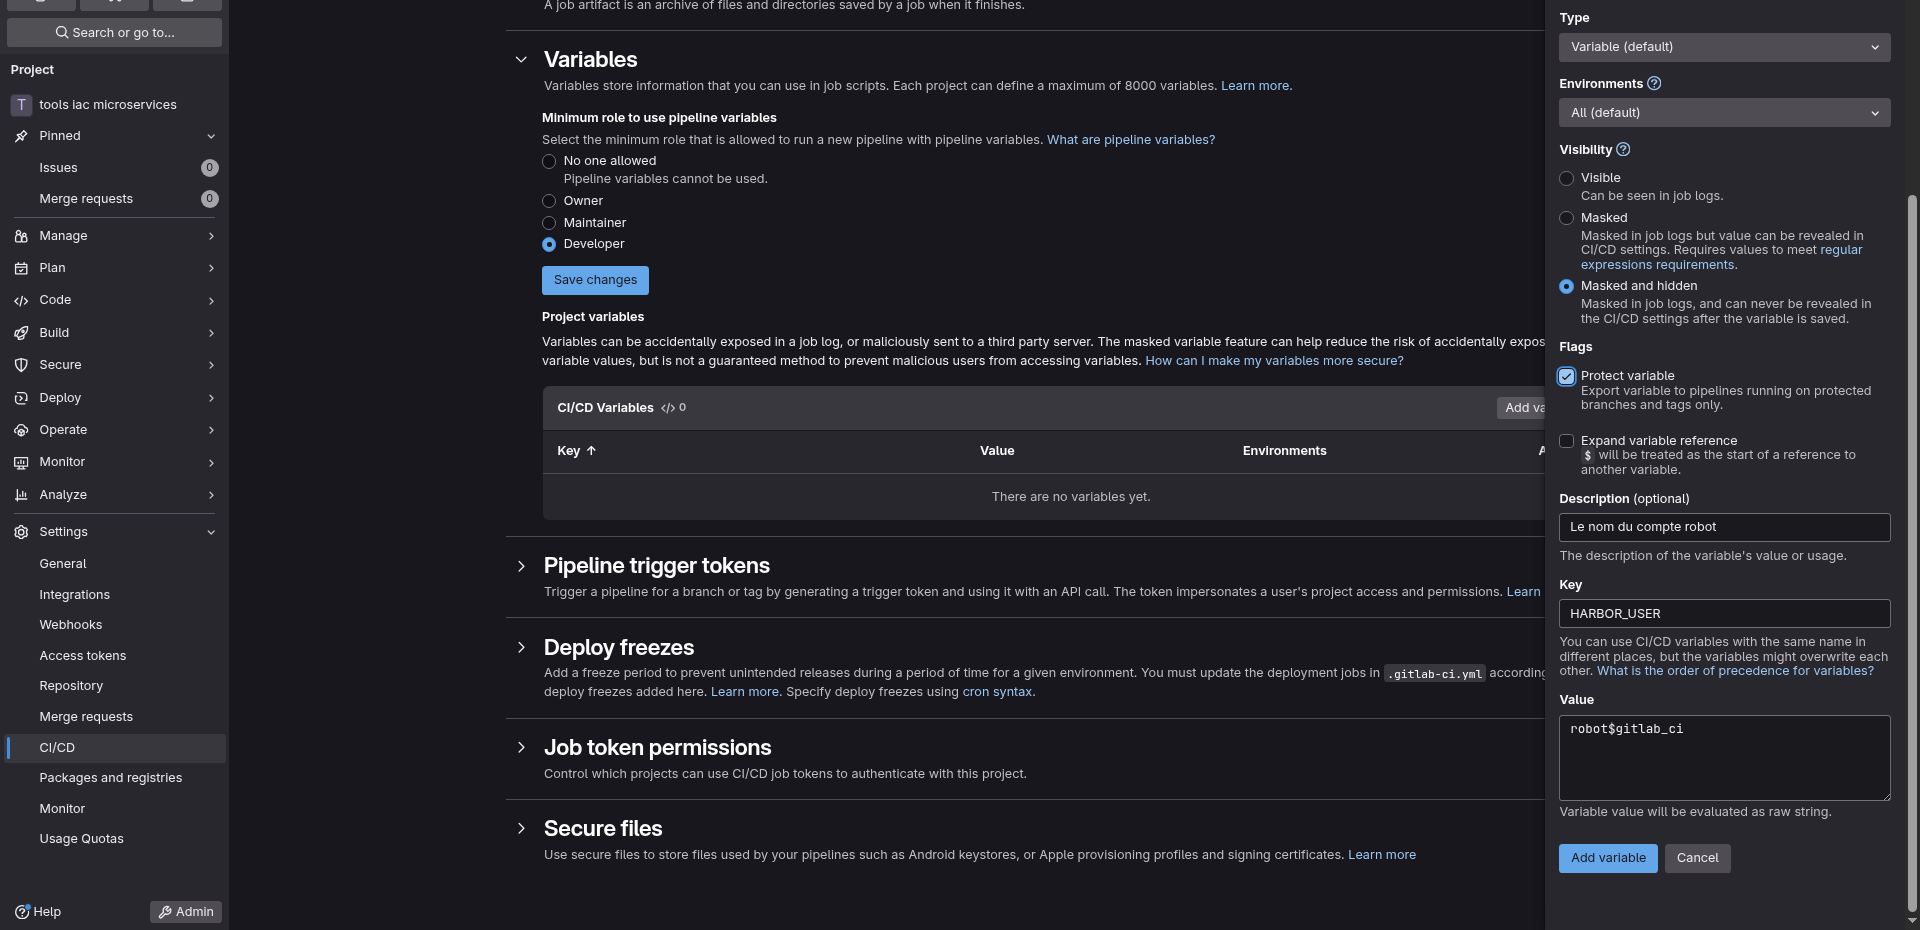
\includegraphics[width=0.65\textwidth]{figures/gitlab variables creation.png}
	\caption{Création et configuration des variables d’environnement pour Harbor}
\end{figure}

Après la définition des variables, le fichier \texttt{.gitlab-ci.yml} a été adapté afin d’inclure une étape d’authentification au registre Harbor avant le push des images Docker. Cette étape est réalisée en injectant les variables d’environnement dans le script d’exécution. L’exemple suivant présente un extrait représentatif de la configuration :

\begin{lstlisting}[caption={Exemple de configuration GitLab CI pour push dans Harbor}]
stages:
  - build
  - push

build_image:
  stage: build
  image: docker:latest
  services:
    - docker:dind
  script:
    - docker build -t $HARBOR_REGISTRY/$HARBOR_PROJECT/my-application:$CI_COMMIT_SHORT_SHA .
    - echo $HARBOR_TOKEN | docker login $HARBOR_REGISTRY -u $HARBOR_USER --password-stdin
    - docker push $HARBOR_REGISTRY/$HARBOR_PROJECT/my-application:$CI_COMMIT_SHORT_SHA
  only:
    - main
\end{lstlisting}

Dans cet exemple :
\begin{itemize}
	\item \texttt{HARBOR\_REGISTRY} désigne l’URL du registre Harbor (par exemple \texttt{harbor.example.com}).
	\item \texttt{HARBOR\_PROJECT} correspond au nom du projet Harbor ciblé.
\end{itemize}

La commande \texttt{docker login} est exécutée avec l’option \texttt{--password-stdin}, permettant de transmettre le jeton sans qu’il apparaisse en clair dans les logs du pipeline. Ce mécanisme contribue à renforcer la sécurité des informations sensibles et à éviter toute fuite accidentelle.

Une fois configuré, le GitLab Runner est en mesure de procéder automatiquement à l’authentification, au build et au push des images Docker vers le registre Harbor. Ce processus est illustré dans le schéma suivant :

\begin{figure}[H]
	\centering
	\begin{tikzpicture} [node distance=2.8cm, auto, thick]

		% Nodes
		\node[draw, rounded corners, minimum width=3.5cm, minimum height=1cm, fill=gray!10] (gitlab) {GitLab CI/CD};

		\node[
			draw,
			rounded corners,
			minimum width=3.5cm,
			minimum height=1cm,
			fill=gray!10,
			right=7cm of gitlab
		] (harbor) {Harbor Registry};

		\node[draw, rounded corners, minimum width=3.5cm, minimum height=1cm, fill=gray!10, below of=gitlab] (runner) {GitLab Runner};

		% Docker image
		\node[draw, rectangle, minimum width=2.5cm, minimum height=0.8cm, fill=blue!5, below of=runner] (image) {Image Docker};

		% Arrows
		\draw[->] (gitlab) -- node[midway, above]{Déclenchement du pipeline} (runner);
		\draw[->] (runner) -- node[midway, left]{docker build} (image);
		\draw[->] (runner.east) -- ++(2.0,0) |- node[pos=0.25, above]{docker login} (harbor.west);
		\draw[->] (image.east) -- ++(2.0,0) |- node[pos=0.25, below]{docker push} (harbor.west);

		% Tokens
		\node[
			rectangle,
			fill=yellow!20,
			draw,
			rounded corners,
			font=\footnotesize,
			below=2cm of harbor,
			align=center
		] (token) {Compte robot\\ \texttt{robot\$gitlab\_ci}\\ Jeton d’authentification};

		\draw[dashed, ->] (token.north) -- (harbor.south);

	\end{tikzpicture}
	\caption{Flux d’authentification et de publication des images Docker entre GitLab et Harbor}
\end{figure}

\subsection{Authentification Argo CD vers GitLab (dépôt GitOps)}

Argo CD doit accéder au dépôt Git contenant les manifests Kubernetes ou les Helm charts à déployer.

\subparagraph{Étapes de configuration}

\begin{enumerate}
	\item \textbf{Créer un token GitLab} :
	      \begin{itemize}
		      \item Aller dans \emph{GitLab > Preferences > Access Tokens}.
		      \item Définir un token avec les scopes : \texttt{read\_repository}, voire \texttt{write\_repository}.
	      \end{itemize}

	      %   \begin{figure}[H]
	      %   	\centering
	      %   	\includegraphics[width=0.6\textwidth]{figures/gitlab_access_token.png}
	      %   	\caption{Création d’un access token GitLab pour Argo CD}
	      %   \end{figure}

	\item \textbf{Ajouter le dépôt dans Argo CD} :
	      \begin{itemize}
		      \item Via la CLI :
		            \begin{lstlisting}[language=bash]
argocd repo add https://gitlab.com/oneex/gitops-repo.git \
  --username <gitlab-username> \
  --password <access-token>
	      	      \end{lstlisting}
		      \item Ou via l’interface graphique : \emph{Settings > Repositories > Connect Repo using HTTPS}.
	      \end{itemize}

	      %   \begin{figure}[H]
	      %   	\centering
	      %   	\includegraphics[width=0.6\textwidth]{figures/argocd_add_repo.png}
	      %   	\caption{Ajout du dépôt GitOps dans Argo CD}
	      %   \end{figure}

	\item \textbf{(Optionnel) Gestion des credentials via Vault ou SealedSecrets} :
	      \begin{itemize}
		      \item Pour éviter le stockage de secrets dans les manifests ou CRDs.
	      \end{itemize}
\end{enumerate}

\vspace{0.5cm}
Ces mécanismes assurent que seuls les outils autorisés peuvent interagir avec Harbor et les dépôts Git, renforçant la sécurité de la chaîne DevOps tout en maintenant une automatisation fluide et traçable.

\subsection{Préparation des tâches des pipelines}

Les tâches élémentaires des pipelines CI/CD ont été définies de manière modulaire.
Elles incluent notamment :
\begin{itemize}
	\item La phase de compilation et de tests unitaires.
	\item La construction des images Docker.
	\item Le scan de sécurité (par exemple avec Trivy) pour détecter les vulnérabilités connues.
	\item La validation syntaxique des manifests Kubernetes (linting).
	\item La mise en cache des dépendances pour accélérer les builds.
\end{itemize}

Chaque tâche est décrite dans un fichier YAML de pipeline et peut être exécutée indépendamment, favorisant la réutilisation entre projets.

\subsection{Préparation des pipelines}

Enfin, les pipelines complets ont été structurés et versionnés dans les dépôts Git des applications.
Ces pipelines définissent :
\begin{itemize}
	\item Les déclencheurs automatiques (push sur la branche principale, création d’une release, merge request).
	\item Les variables d’environnement spécifiques à chaque environnement cible (dev, recette, production).
	\item Les étapes de build, de test, de publication et de déploiement continu.
	\item Les conditions de déclenchement manuel ou automatique de certaines étapes sensibles (par exemple le déploiement en production).
\end{itemize}

L’ensemble du processus CI/CD permet ainsi de passer d’un simple commit de code source jusqu’à la mise à jour des pods Kubernetes de façon totalement automatisée et traçable.

\section{Introduction à l’observabilité}

L’observabilité constitue un pilier essentiel dans la gestion moderne des systèmes distribués. Elle regroupe l’ensemble des pratiques, outils et processus permettant de comprendre le comportement d’une infrastructure, de détecter les anomalies et de garantir la conformité aux exigences de sécurité et de qualité de service.

Dans le contexte des architectures conteneurisées et des microservices, la complexité opérationnelle s’est fortement accrue. Chaque requête peut transiter par de nombreux composants, rendant le diagnostic des incidents particulièrement difficile sans outils adaptés.

Par ailleurs, les exigences réglementaires et les bonnes pratiques imposent de disposer d’audits précis des accès, des changements et des événements critiques. L’observabilité et l’audit ne se limitent donc pas à la simple surveillance technique, mais participent également à la gouvernance et à la gestion des risques.

Enfin, il est important de souligner que surveiller uniquement des métriques brutes telles que l’utilisation CPU ou mémoire (« CPU à 80 \% », par exemple) n’est pas suffisant. Ces indicateurs doivent être replacés dans leur contexte et enrichis par des analyses plus poussées (traçage distribué, corrélation d’événements, détection d’anomalies, etc.), comme nous le verrons dans les chapitres suivants.

\subsection{Contexte et enjeux de l'observabilité et de l'audit}

La mise en place d’un dispositif d’observabilité répond à plusieurs enjeux majeurs :

\begin{itemize}
	\item \textbf{Diagnostic rapide des incidents} : être capable de reconstituer le scénario précis ayant conduit à une panne ou à un comportement inattendu.
	\item \textbf{Optimisation des performances} : mesurer et analyser les temps de réponse, l’utilisation des ressources et la saturation éventuelle des composants.
	\item \textbf{Sécurité et traçabilité} : enregistrer les accès, les tentatives d’intrusion et les changements de configuration, afin de disposer de preuves en cas d’incident de sécurité.
	\item \textbf{Conformité réglementaire} : répondre aux obligations légales ou contractuelles en matière de conservation des journaux et de traçabilité des actions (par exemple, RGPD, ANSII, ISO 27001).
	\item \textbf{Amélioration continue} : exploiter les données collectées pour identifier les points faibles et guider les évolutions de l’architecture.
	\item \textbf{Garantie d’un meilleur SLA} : offrir aux utilisateurs un niveau de service mesurable et prévisible (disponibilité, performance, temps de rétablissement), en s’appuyant sur des indicateurs objectifs qui permettent de suivre et démontrer le respect des engagements contractuels.
\end{itemize}

Dans le cadre de ce projet, l’objectif est de fournir une visibilité unifiée sur l’état de l’infrastructure Kubernetes, des services applicatifs et des flux réseau, en s’appuyant sur des outils open source et des processus automatisés.

\section{Outils de supervision et tendances}

L’état de l’art de l’observabilité se structure autour de trois piliers principaux, souvent désignés sous l’acronyme \textbf{MELT} (Metrics, Events, Logs, Traces) :

\begin{enumerate}
	\item \textbf{Les métriques} : valeurs numériques collectées à intervalles réguliers (CPU, mémoire, latence). Des solutions comme Prometheus ou InfluxDB permettent de stocker et d’interroger ces mesures.
	\item \textbf{Les événements et alertes} : notifications déclenchées par un seuil ou un changement d’état. Ces événements sont souvent gérés par Alertmanager ou des systèmes de gestion d’incidents (PagerDuty, Opsgenie).
	\item \textbf{Les logs} : traces textuelles produites par les applications et les composants système. Les solutions modernes (Elastic Stack, Loki) facilitent la collecte et la recherche en temps réel.
	\item \textbf{Les traces distribuées} : enregistrements du parcours d’une requête à travers les microservices. Des outils comme Jaeger et OpenTelemetry sont devenus des standards de facto.
\end{enumerate}

Les tendances actuelles mettent en avant plusieurs évolutions :

\begin{itemize}
	\item \textbf{L’adoption massive de l’open source} : la plupart des organisations privilégient des solutions libres et communautaires pour éviter l’enfermement propriétaire.
	\item \textbf{Le modèle as-a-Service} : de nombreux acteurs (Datadog, New Relic, Grafana Cloud) proposent des plateformes hébergées intégrant l’ensemble des fonctionnalités d’observabilité.
	\item \textbf{La convergence des données} : les métriques, logs et traces ne sont plus traités isolément mais regroupés dans des plateformes unifiées facilitant les corrélations.
	\item \textbf{L’intégration avec GitOps et l’automatisation} : les configurations de monitoring et d’alerting sont versionnées et déployées de la même manière que les ressources Kubernetes.
	\item \textbf{La montée en puissance d’OpenTelemetry} : ce projet CNCF s’impose comme le standard unique de collecte de la télémétrie dans les environnements cloud-native.
\end{itemize}

Ces évolutions permettent de construire des systèmes plus résilients, plus sécurisés et plus faciles à maintenir, tout en apportant une meilleure compréhension globale des environnements complexes.

\subsection{Grafana}

Grafana est une solution open source de visualisation et d’exploration de données, largement utilisée pour la supervision des infrastructures, le monitoring applicatif et l’analyse d’indicateurs métiers. Elle permet de créer des tableaux de bord interactifs et personnalisables qui agrègent des données provenant de multiples sources (Prometheus, InfluxDB, Elasticsearch, Loki, MySQL, etc.). Grâce à son approche modulaire et à sa richesse fonctionnelle, Grafana s’est imposé comme un standard de facto dans l’écosystème cloud-native et DevOps.

%point de vue metier
Grafana répond à plusieurs enjeux stratégiques  : renforcer la visibilité sur les systèmes critiques, réduire le temps de résolution des incidents, et améliorer la qualité des services. En centralisant la visualisation et l’analyse des métriques, logs et traces, Grafana facilite la prise de décision et contribue à l’amélioration continue des processus opérationnels. Son interface conviviale et ses capacités de partage simplifient la collaboration entre équipes techniques et parties prenantes.

%point de vue logique et technique
, Grafana repose sur plusieurs composants essentiels  :
\begin{itemize}
	\item \textbf{Les datasources}  : connecteurs vers des bases de données et des systèmes de monitoring (Prometheus, Graphite, ElasticSearch, CloudWatch, etc.).
	\item \textbf{Les dashboards}  : ensembles de panels configurables qui visualisent les données sous forme de graphiques, jauges, tableaux et alertes.
	\item \textbf{Les panels}  : éléments de visualisation individuels, paramétrés avec des requêtes, des transformations et des styles personnalisés.
	\item \textbf{Les alertes}  : règles qui surveillent les seuils définis et déclenchent des notifications en cas d’anomalie.
	\item \textbf{Les organisations et utilisateurs}  : système de gestion des accès, des permissions et des partages.
\end{itemize}

Grafana peut être déployé en standalone ou intégré dans des stacks d’observabilité complètes (exemple  : Prometheus + Loki + Grafana). Son API REST et son support des plugins en font un outil particulièrement extensible et adaptable à tous les cas d’usage.

\textbf{Exemples et cas d’usage} :
\begin{itemize}
	\item Visualiser en temps réel les métriques d’un cluster Kubernetes (CPU, mémoire, pods, etc.) en s’appuyant sur Prometheus.
	\item Corréler les logs applicatifs via Loki avec les indicateurs de performance pour diagnostiquer plus rapidement un incident.
	\item Configurer des alertes pour notifier les équipes DevOps en cas de dépassement d’un seuil critique (ex. latence élevée).
	\item Créer des tableaux de bord métiers synthétiques avec des indicateurs clés (KPI) accessibles aux décideurs.
	\item Intégrer Grafana avec Slack ou PagerDuty pour centraliser les alertes et les escalades.
\end{itemize}

\textbf{Avantages principaux} :
\begin{itemize}
	\item Plateforme unifiée de visualisation multi-sources et multi-formats.
	\item Interface ergonomique et hautement personnalisable.
	\item Large écosystème de plugins, dashboards communautaires et connecteurs.
	\item Support des alertes natives et intégration avec les systèmes de notification.
	\item Extensibilité via API REST, provisioning as code et gestion des permissions fine.
	\item Solution open source mature, supportée par une large communauté.
\end{itemize}

En synthèse, Grafana est une brique centrale des stratégies d’observabilité modernes. Il permet aux organisations de transformer leurs données en connaissances actionnables, d’améliorer la performance opérationnelle et de renforcer la confiance dans les systèmes distribués.

\textbf{Références suggérées} :
\begin{itemize}
	\item Grafana Documentation – \url{https://grafana.com/docs/}
	\item Grafana GitHub Repository – \url{https://github.com/grafana/grafana}
	\item Prometheus Documentation – \url{https://prometheus.io/docs/}
	\item Loki Documentation – \url{https://grafana.com/docs/loki/latest/}
	\item Grafana Labs Blog – \url{https://grafana.com/blog/}
\end{itemize}

\subsection{Prometheus}

Prometheus est une solution open source de monitoring et d’alerte initialement développée par SoundCloud, puis incubée par la Cloud Native Computing Foundation (CNCF). Il est devenu l’un des piliers des architectures cloud-native grâce à sa capacité à collecter, stocker et interroger des métriques temporelles de manière performante. Prometheus est particulièrement reconnu pour son modèle de données multidimensionnel, son langage de requête puissant (PromQL) et sa facilité d’intégration avec Kubernetes.

%point de vue metier
Prometheus répond à plusieurs enjeux essentiels  : renforcer la visibilité sur les systèmes critiques, anticiper les incidents par une surveillance proactive et réduire le temps moyen de résolution des problèmes (MTTR). Il contribue à l’amélioration continue des performances applicatives et à la qualité de service délivrée aux utilisateurs. Grâce à sa modularité, Prometheus s’adapte à des environnements variés (infrastructures cloud, conteneurs, clusters Kubernetes, applications legacy).

%point de vue logique et technique
, Prometheus repose sur plusieurs composants clés  :
\begin{itemize}
	\item \textbf{Le serveur Prometheus}  : responsable de la collecte des métriques via le protocole HTTP/HTTPS (pull model) et du stockage local des séries temporelles.
	\item \textbf{Les exporters}  : processus ou agents qui exposent des métriques au format Prometheus (ex.: Node Exporter, Blackbox Exporter, MySQL Exporter).
	\item \textbf{Le langage PromQL}  : langage de requête permettant d’agréger, filtrer et analyser les métriques.
	\item \textbf{Les règles d’alerte}  : expressions PromQL évaluées en continu pour générer des alertes.
	\item \textbf{Alertmanager}  : composant dédié à la gestion et au routage des alertes vers les canaux de notification (email, Slack, PagerDuty).
\end{itemize}

Prometheus est particulièrement bien intégré dans l’écosystème Kubernetes grâce à la découverte de services automatique, facilitant ainsi la supervision des clusters et des workloads dynamiques.

\textbf{Exemples et cas d’usage} :
\begin{itemize}
	\item Superviser l’utilisation CPU et mémoire des nœuds Kubernetes via Node Exporter.
	\item Mesurer la latence et le taux d’erreurs des endpoints HTTP exposés par des microservices.
	\item Définir une alerte déclenchée lorsque la disponibilité d’un service passe sous un seuil critique.
	\item Stocker des métriques de performance applicative pour des analyses historiques.
	\item Visualiser les métriques dans Grafana grâce au connecteur natif Prometheus.
\end{itemize}

\textbf{Avantages principaux} :
\begin{itemize}
	\item Modèle de collecte pull simplifiant l’intégration avec les workloads dynamiques.
	\item Stockage en séries temporelles optimisé pour la performance et la rétention longue durée.
	\item Langage PromQL expressif et puissant pour l’analyse des données.
	\item Intégration native avec Kubernetes et les architectures cloud-native.
	\item Écosystème riche d’exporters et de dashboards communautaires.
	\item Solution open source mature, soutenue par la CNCF et une large communauté.
\end{itemize}

En synthèse, Prometheus est un outil incontournable des stratégies de monitoring et d’observabilité modernes. Il apporte robustesse, flexibilité et transparence à la supervision des infrastructures complexes et des applications distribuées.

\textbf{Références suggérées} :
\begin{itemize}
	\item Prometheus Documentation – \url{https://prometheus.io/docs/}
	\item Prometheus GitHub Repository – \url{https://github.com/prometheus/prometheus}
	\item CNCF Prometheus Project – \url{https://www.cncf.io/projects/prometheus/}
	\item Grafana Documentation – \url{https://grafana.com/docs/grafana/latest/datasources/prometheus/}
	\item Monitoring with Prometheus – James Turnbull. O’Reilly Media.
\end{itemize}

\subsection{Loki}

Loki est une solution open source développée par Grafana Labs pour la centralisation et l’analyse des logs. Conçu pour s’intégrer étroitement avec Prometheus, Grafana et l’écosystème cloud-native, Loki adopte une approche innovante  : il indexe uniquement les labels (métadonnées) et non le contenu complet des logs. Cette caractéristique en fait une solution plus légère, plus scalable et plus économique que les systèmes traditionnels d’indexation complète (par exemple Elasticsearch).

%point de vue metier
Loki répond à plusieurs enjeux stratégiques  : renforcer la visibilité sur les applications et les infrastructures, accélérer les diagnostics d’incidents et réduire le coût du stockage et du traitement des logs. Il permet aux équipes SRE, DevOps et de support de disposer d’un outil cohérent avec leur stack de monitoring et d’observabilité, facilitant la corrélation entre métriques, logs et alertes.

%point de vue logique et technique
, Loki repose sur plusieurs concepts clés  :
\begin{itemize}
	\item \textbf{Les labels}  : clés et valeurs attachées aux streams de logs (par exemple `app="nginx"`), utilisés comme index.
	\item \textbf{Les chunks}  : segments de données compressées regroupant les logs non indexés.
	\item \textbf{Promtail}  : agent qui collecte les logs sur les hôtes et les envoie à Loki.
	\item \textbf{Le langage LogQL}  : langage de requête inspiré de PromQL, permettant d’interroger et d’agréger les logs.
	\item \textbf{L’intégration Grafana}  : visualisation et exploration des logs dans des dashboards unifiés.
\end{itemize}

Grâce à sa compatibilité Kubernetes et à sa scalabilité horizontale, Loki est particulièrement adapté aux environnements cloud-native et microservices.

\textbf{Exemples et cas d’usage} :
\begin{itemize}
	\item Collecter les logs des conteneurs Kubernetes via Promtail et les regrouper par namespace, pod et container.
	\item Corréler des pics de latence observés dans Prometheus avec les logs applicatifs de la même période.
	\item Configurer une alerte Grafana qui affiche les logs d’erreurs critiques lors d’un incident.
	\item Archiver les logs applicatifs de manière compressée et économique sur le long terme.
	\item Rechercher rapidement les logs d’un service particulier via LogQL.
\end{itemize}

\textbf{Avantages principaux} :
\begin{itemize}
	\item Scalabilité horizontale et stockage économique grâce à l’indexation minimale.
	\item Intégration native avec Grafana et Prometheus.
	\item Requêtes puissantes et flexibles avec LogQL.
	\item Support complet de Kubernetes et des environnements multi-cloud.
	\item Solution open source mature et soutenue par une large communauté.
\end{itemize}

En synthèse, Loki est un composant central de la stack d’observabilité cloud-native. Il permet aux organisations de simplifier et de rationaliser la gestion des logs, tout en réduisant les coûts et en améliorant la capacité de diagnostic et de supervision.

\textbf{Références suggérées} :
\begin{itemize}
	\item Loki Documentation – \url{https://grafana.com/docs/loki/latest/}
	\item Loki GitHub Repository – \url{https://github.com/grafana/loki}
	\item Grafana Documentation – \url{https://grafana.com/docs/}
	\item Promtail Documentation – \url{https://grafana.com/docs/loki/latest/clients/promtail/}
	\item CNCF Loki Project – \url{https://www.cncf.io/projects/loki/}
\end{itemize}

\subsection{Tempo}

Tempo est une solution open source de traçage distribué développée par Grafana Labs. Elle permet de collecter, stocker et interroger des traces issues d’applications distribuées, sans nécessiter d’indexation complexe. Conçu pour compléter Prometheus et Loki, Tempo s’intègre naturellement dans la stack d’observabilité cloud-native. Grâce à son architecture optimisée, il offre un stockage massif et économique des traces, tout en simplifiant la corrélation avec les métriques et les logs.

%point de vue metier
Tempo répond à plusieurs enjeux stratégiques  : comprendre la performance des applications microservices, diagnostiquer les latences et les erreurs en production, et améliorer l’expérience utilisateur. En facilitant l’analyse des parcours complets des requêtes, Tempo contribue à réduire le temps moyen de résolution des incidents (MTTR) et à optimiser la qualité de service.

%point de vue logique et technique
, Tempo s’appuie sur plusieurs concepts essentiels  :
\begin{itemize}
	\item \textbf{Les traces}  : enregistrements d’un ensemble de spans représentant les étapes d’une requête distribuée.
	\item \textbf{Les spans}  : unités atomiques contenant les métadonnées sur chaque étape (durée, étiquettes, événements).
	\item \textbf{L’ingester}  : composant qui reçoit et stocke les traces dans des blocs compressés.
	\item \textbf{L’indexation minimale}  : Tempo utilise un modèle «  No Index  », reposant uniquement sur l’identifiant de trace, ce qui simplifie le stockage et réduit les coûts.
	\item \textbf{L’intégration avec Grafana}  : Tempo permet de visualiser et de rechercher les traces via l’interface Grafana, en corrélation avec les métriques Prometheus et les logs Loki.
\end{itemize}

Tempo est compatible avec les formats de traçage standardisés comme OpenTelemetry, Jaeger et Zipkin, facilitant l’intégration avec un grand nombre de frameworks et de langages.

\textbf{Exemples et cas d’usage} :
\begin{itemize}
	\item Collecter les traces d’une application microservices instrumentée avec OpenTelemetry.
	\item Corréler un pic de latence observé dans Prometheus avec les traces détaillant les appels entre services.
	\item Rechercher des traces via leur identifiant unique depuis un log collecté par Loki.
	\item Visualiser les dépendances entre services et la durée de chaque étape d’une requête.
	\item Conserver l’historique des traces pour analyse et optimisation des performances applicatives.
\end{itemize}

\textbf{Avantages principaux} :
\begin{itemize}
	\item Scalabilité horizontale et stockage économique sans indexation complexe.
	\item Compatibilité native avec OpenTelemetry, Jaeger et Zipkin.
	\item Corrélation simple avec les métriques et logs via Grafana.
	\item Facilité de déploiement dans des environnements Kubernetes et cloud.
	\item Solution open source soutenue par la CNCF et Grafana Labs.
\end{itemize}

En synthèse, Tempo est un pilier des architectures d’observabilité modernes. Il apporte visibilité, compréhension et capacité de diagnostic sur les systèmes distribués, en complément parfait de Prometheus et Loki.

\textbf{Références suggérées} :
\begin{itemize}
	\item Tempo Documentation – \url{https://grafana.com/docs/tempo/latest/}
	\item Tempo GitHub Repository – \url{https://github.com/grafana/tempo}
	\item OpenTelemetry Documentation – \url{https://opentelemetry.io/docs/}
	\item Jaeger Documentation – \url{https://www.jaegertracing.io/docs/}
	\item Grafana Labs Blog – \url{https://grafana.com/blog/}
\end{itemize}

% \subsection{OpenTelemetry}

% OpenTelemetry est une suite open source de spécifications, d’outils et de SDK destinée à la collecte, au traitement et à l’exportation des signaux d’observabilité  : métriques, logs et traces. Né de la fusion des projets OpenTracing et OpenCensus, OpenTelemetry est aujourd’hui un projet de la Cloud Native Computing Foundation (CNCF) et constitue le standard de facto pour instrumenter les applications modernes, qu’elles soient monolithiques ou microservices.

% %point de vue metier
% OpenTelemetry répond à des enjeux stratégiques majeurs  : renforcer la visibilité sur les systèmes distribués, anticiper les problèmes de performance, améliorer l’expérience utilisateur et faciliter la transformation digitale. En proposant un cadre unifié et standardisé, OpenTelemetry contribue à réduire la complexité opérationnelle et à accélérer la mise en place de stratégies d’observabilité efficaces.

% %point de vue logique et technique
% , OpenTelemetry repose sur plusieurs composants essentiels  :
% \begin{itemize}
% 	\item \textbf{Les SDK}  : bibliothèques spécifiques aux langages (Java, Go, Python, etc.) qui instrumentent automatiquement ou manuellement les applications.
% 	\item \textbf{Le Collector}  : service qui reçoit, traite et exporte les signaux vers des backends comme Prometheus, Jaeger, Tempo, Zipkin ou Grafana.
% 	\item \textbf{Les exporters}  : composants qui envoient les données collectées vers des systèmes tiers.
% 	\item \textbf{Les ressources}  : ensembles de métadonnées qui décrivent les attributs des services (nom, version, environnement).
% 	\item \textbf{Les protocoles}  : principalement OTLP (OpenTelemetry Protocol), conçu pour un transport efficace et interopérable des signaux.
% \end{itemize}

% OpenTelemetry est conçu comme un projet modulaire et extensible, permettant aux équipes d’adopter progressivement la collecte des traces, des métriques et des logs, selon leurs priorités.

% \textbf{Exemples et cas d’usage} :
% \begin{itemize}
% 	\item Instrumenter automatiquement une API REST en Java pour collecter les latences et les erreurs.
% 	\item Exporter les métriques applicatives vers Prometheus et les traces vers Tempo via le Collector.
% 	\item Corréler les logs et les traces grâce à des identifiants de corrélation injectés automatiquement.
% 	\item Visualiser le graphe de dépendances entre microservices dans Jaeger ou Grafana.
% 	\item Monitorer en temps réel les indicateurs de performance d’un cluster Kubernetes.
% \end{itemize}

% \textbf{Avantages principaux} :
% \begin{itemize}
% 	\item Standardisation des signaux d’observabilité (métriques, traces, logs).
% 	\item Large compatibilité multi-langages et multi-plateformes.
% 	\item Collecte et exportation flexibles via le Collector.
% 	\item Intégration fluide avec les principaux backends d’observabilité.
% 	\item Support actif par une large communauté et les principaux éditeurs cloud.
% 	\item Réduction de la complexité opérationnelle et meilleure visibilité end-to-end.
% \end{itemize}

% En synthèse, OpenTelemetry est une brique fondamentale de l’observabilité moderne. Il offre un cadre unifié, extensible et standardisé, permettant aux organisations de mieux comprendre et améliorer le comportement de leurs applications distribuées.

% \textbf{Références suggérées} :
% \begin{itemize}
% 	\item OpenTelemetry Documentation – \url{https://opentelemetry.io/docs/}
% 	\item OpenTelemetry GitHub – \url{https://github.com/open-telemetry/opentelemetry-specification}
% 	\item CNCF OpenTelemetry Project – \url{https://www.cncf.io/projects/opentelemetry/}
% 	\item Jaeger Documentation – \url{https://www.jaegertracing.io/docs/}
% 	\item Grafana Tempo Documentation – \url{https://grafana.com/docs/tempo/latest/}
% \end{itemize}

\section{Mise en place du monitoring continu}

La mise en place du monitoring continu est indispensable pour assurer la supervision proactive de l’infrastructure et des applications.
Le projet s’appuie principalement sur la solution Prometheus, qui collecte les métriques exposées par les composants Kubernetes et les services applicatifs via des endpoints HTTP (\texttt{/metrics}).

Les étapes principales comprennent :
\begin{itemize}
	\item Le déploiement de l’opérateur Prometheus dans le cluster Kubernetes.
	\item La définition des \texttt{ServiceMonitor} et \texttt{PodMonitor} permettant de déclarer les cibles à surveiller.
	\item La configuration des règles d’alerting basées sur les métriques collectées.
	\item L’intégration avec Grafana pour la visualisation en temps réel des tableaux de bord.
\end{itemize}

Grâce à cette approche, l’état des systèmes est suivi en continu et les anomalies peuvent être détectées de manière précoce.

\section{Gestion des alertes et des incidents}

La gestion des alertes repose sur l’utilisation de Prometheus Alertmanager.
Ce composant reçoit les alertes générées par Prometheus selon les règles prédéfinies (par exemple seuils de charge CPU, absence de pods, erreurs applicatives).

Les principaux éléments mis en place sont :
\begin{itemize}
	\item La configuration des routes d’alerte permettant d’acheminer les notifications vers les destinataires appropriés (e-mails, canaux Slack, systèmes d’escalade).
	\item La définition des silences pour désactiver temporairement des alertes lors de maintenances planifiées.
	\item L’organisation des alertes par sévérité et par environnement (développement, recette, production).
	\item La documentation des procédures de réponse aux incidents.
\end{itemize}

Ce dispositif contribue à réduire le temps moyen de résolution des incidents et à limiter leur impact sur les utilisateurs.

\section{Gestion des logs}

La collecte centralisée des logs est un pilier de l’observabilité.
Dans ce projet, la stack EFK (Elasticsearch, Fluentd, Kibana) ou Loki a été utilisée afin d’agréger les journaux produits par :
\begin{itemize}
	\item Les pods Kubernetes.
	\item Les composants système des nœuds.
	\item Les applications déployées.
\end{itemize}

Les principales fonctionnalités implémentées sont :
\begin{itemize}
	\item La normalisation et l’enrichissement des logs avec des métadonnées Kubernetes (namespace, nom du pod, labels).
	\item L’indexation et la conservation des journaux selon des politiques de rétention définies.
	\item La recherche en temps réel et la création de tableaux de bord personnalisés dans Kibana ou Grafana.
	\item La détection automatique d’événements critiques et la génération de notifications.
\end{itemize}

Cette centralisation des logs permet de gagner en efficacité lors des diagnostics et de garantir la traçabilité complète des événements.

\section{Gestion des traces distribuées}

Les traces distribuées apportent une vision fine du parcours des requêtes à travers les différents microservices.
Le projet s’appuie sur la suite OpenTelemetry pour instrumenter les applications et collecter les traces.

Les éléments mis en œuvre sont :
\begin{itemize}
	\item L’instrumentation automatique et manuelle du code pour générer des spans et propager le contexte de trace.
	\item Le déploiement du collector OpenTelemetry dans Kubernetes.
	\item L’export des traces vers un backend comme Jaeger ou Grafana Tempo.
	\item La visualisation des dépendances et des performances des requêtes via des interfaces web dédiées.
\end{itemize}

Les traces permettent notamment de :
\begin{itemize}
	\item Identifier les goulets d’étranglement et les sources de latence.
	\item Suivre l’impact des erreurs sur l’ensemble du parcours utilisateur.
	\item Corréler les traces avec les logs et les métriques.
\end{itemize}

\section{Automatisation des audits et de la conformité}

L’automatisation des audits et de la conformité vise à garantir le respect des exigences réglementaires et des politiques internes.

Pour atteindre cet objectif, plusieurs mesures ont été adoptées :
\begin{itemize}
	\item L’activation de l’audit logging Kubernetes pour enregistrer toutes les requêtes API et changements d’état.
	\item La centralisation des journaux d’audit dans Elasticsearch pour une conservation longue durée et une recherche efficace.
	\item La mise en place de règles de contrôle (OPA/Gatekeeper) validant les configurations déployées (politiques de sécurité, labels obligatoires, restrictions de privilèges).
	\item La génération automatique de rapports de conformité sur les accès et les déploiements.
\end{itemize}

Ces mécanismes facilitent les contrôles internes et externes et contribuent à renforcer la confiance dans la plateforme.